\documentclass{article}

\usepackage{minitoc}
\usepackage{tabularx}
\usepackage{booktabs}
\usepackage{graphicx}
\usepackage{hyperref}
\usepackage{xcolor}
\usepackage{blkarray}
\usepackage{amsthm, amssymb, amsmath}
\usepackage{caption}
\usepackage{subcaption}
\usepackage{multirow}
\usepackage[ruled,vlined]{algorithm2e}

\usepackage{natbib}
\bibliographystyle{abbrvnat}

\theoremstyle{definition}
\newtheorem{definition}{Definition}[section]
\newtheorem{theorem}{Theorem}[section]
\newtheorem{lemma}[theorem]{Lemma}
\newtheorem{conjecture}[theorem]{Conjecture}

\usepackage[margin=2.5cm, includefoot, footskip=30pt]{geometry}
\pagestyle{plain}
\setlength{\parindent}{0em}
\setlength{\parskip}{1em}

\renewcommand{\baselinestretch}{1}

\usepackage{standalone}

\newtheorem{proposition}{Proposition}

\title{$n-$bits reactive strategies}

\author{Nikoleta E. Glynatsi, Ethan Akin, Martin Nowak, Christian Hilbe}
\date{}

\begin{document}

\maketitle


\section{Introduction}

In this work we explore \textit{reactive strategies} in the infinitely repeated
prisoner's dilemma. The prisoner's dilemma is a two person symmetric game that
provides a simple model of cooperation. Each of the two players, \(p\) and
\(q\), simultaneously and independently decide to cooperate (\(C\)) or to defect
(\(D\)). A player who cooperates pays a cost \(c > 0\) to provide a benefit
\(b > c\) for the co-player. A cooperator either gets \(b\!-\!c\) (if the
co-player also cooperates) or \(-c\) (if the co-player defects). Respectively, a defector either gets
\(b\) (if the co-player cooperates) or 0 (if the co-player defects), and so,
the payoffs of player \(p\) take the form,

\begin{equation}\label{eq:donation_payoffs}
  \begin{blockarray}{ccc}
      & \text{cooperate} & \text{defect} \\
      \begin{block}{c(cc)}
          \text{cooperate} & b\!-\!c & -c \\
          \text{defect} & b & 0 \\
      \end{block}
  \end{blockarray}
\end{equation}

The transpose of (\ref{eq:donation_payoffs}) gives the payoffs of co-player
\(q\). We can also define each player's payoffs as vectors,

\begin{equation}\label{eq:vector_payoffs}
  \mathbf{S}_{p} = (b\!-\!c, -c, b, 0) \quad \textrm{and} \quad  \mathbf{S}_{q} = (b\!-\!c, b, -c, 0).
\end{equation}

\section{Model}

\begin{figure}[!htbp]
    \centering
    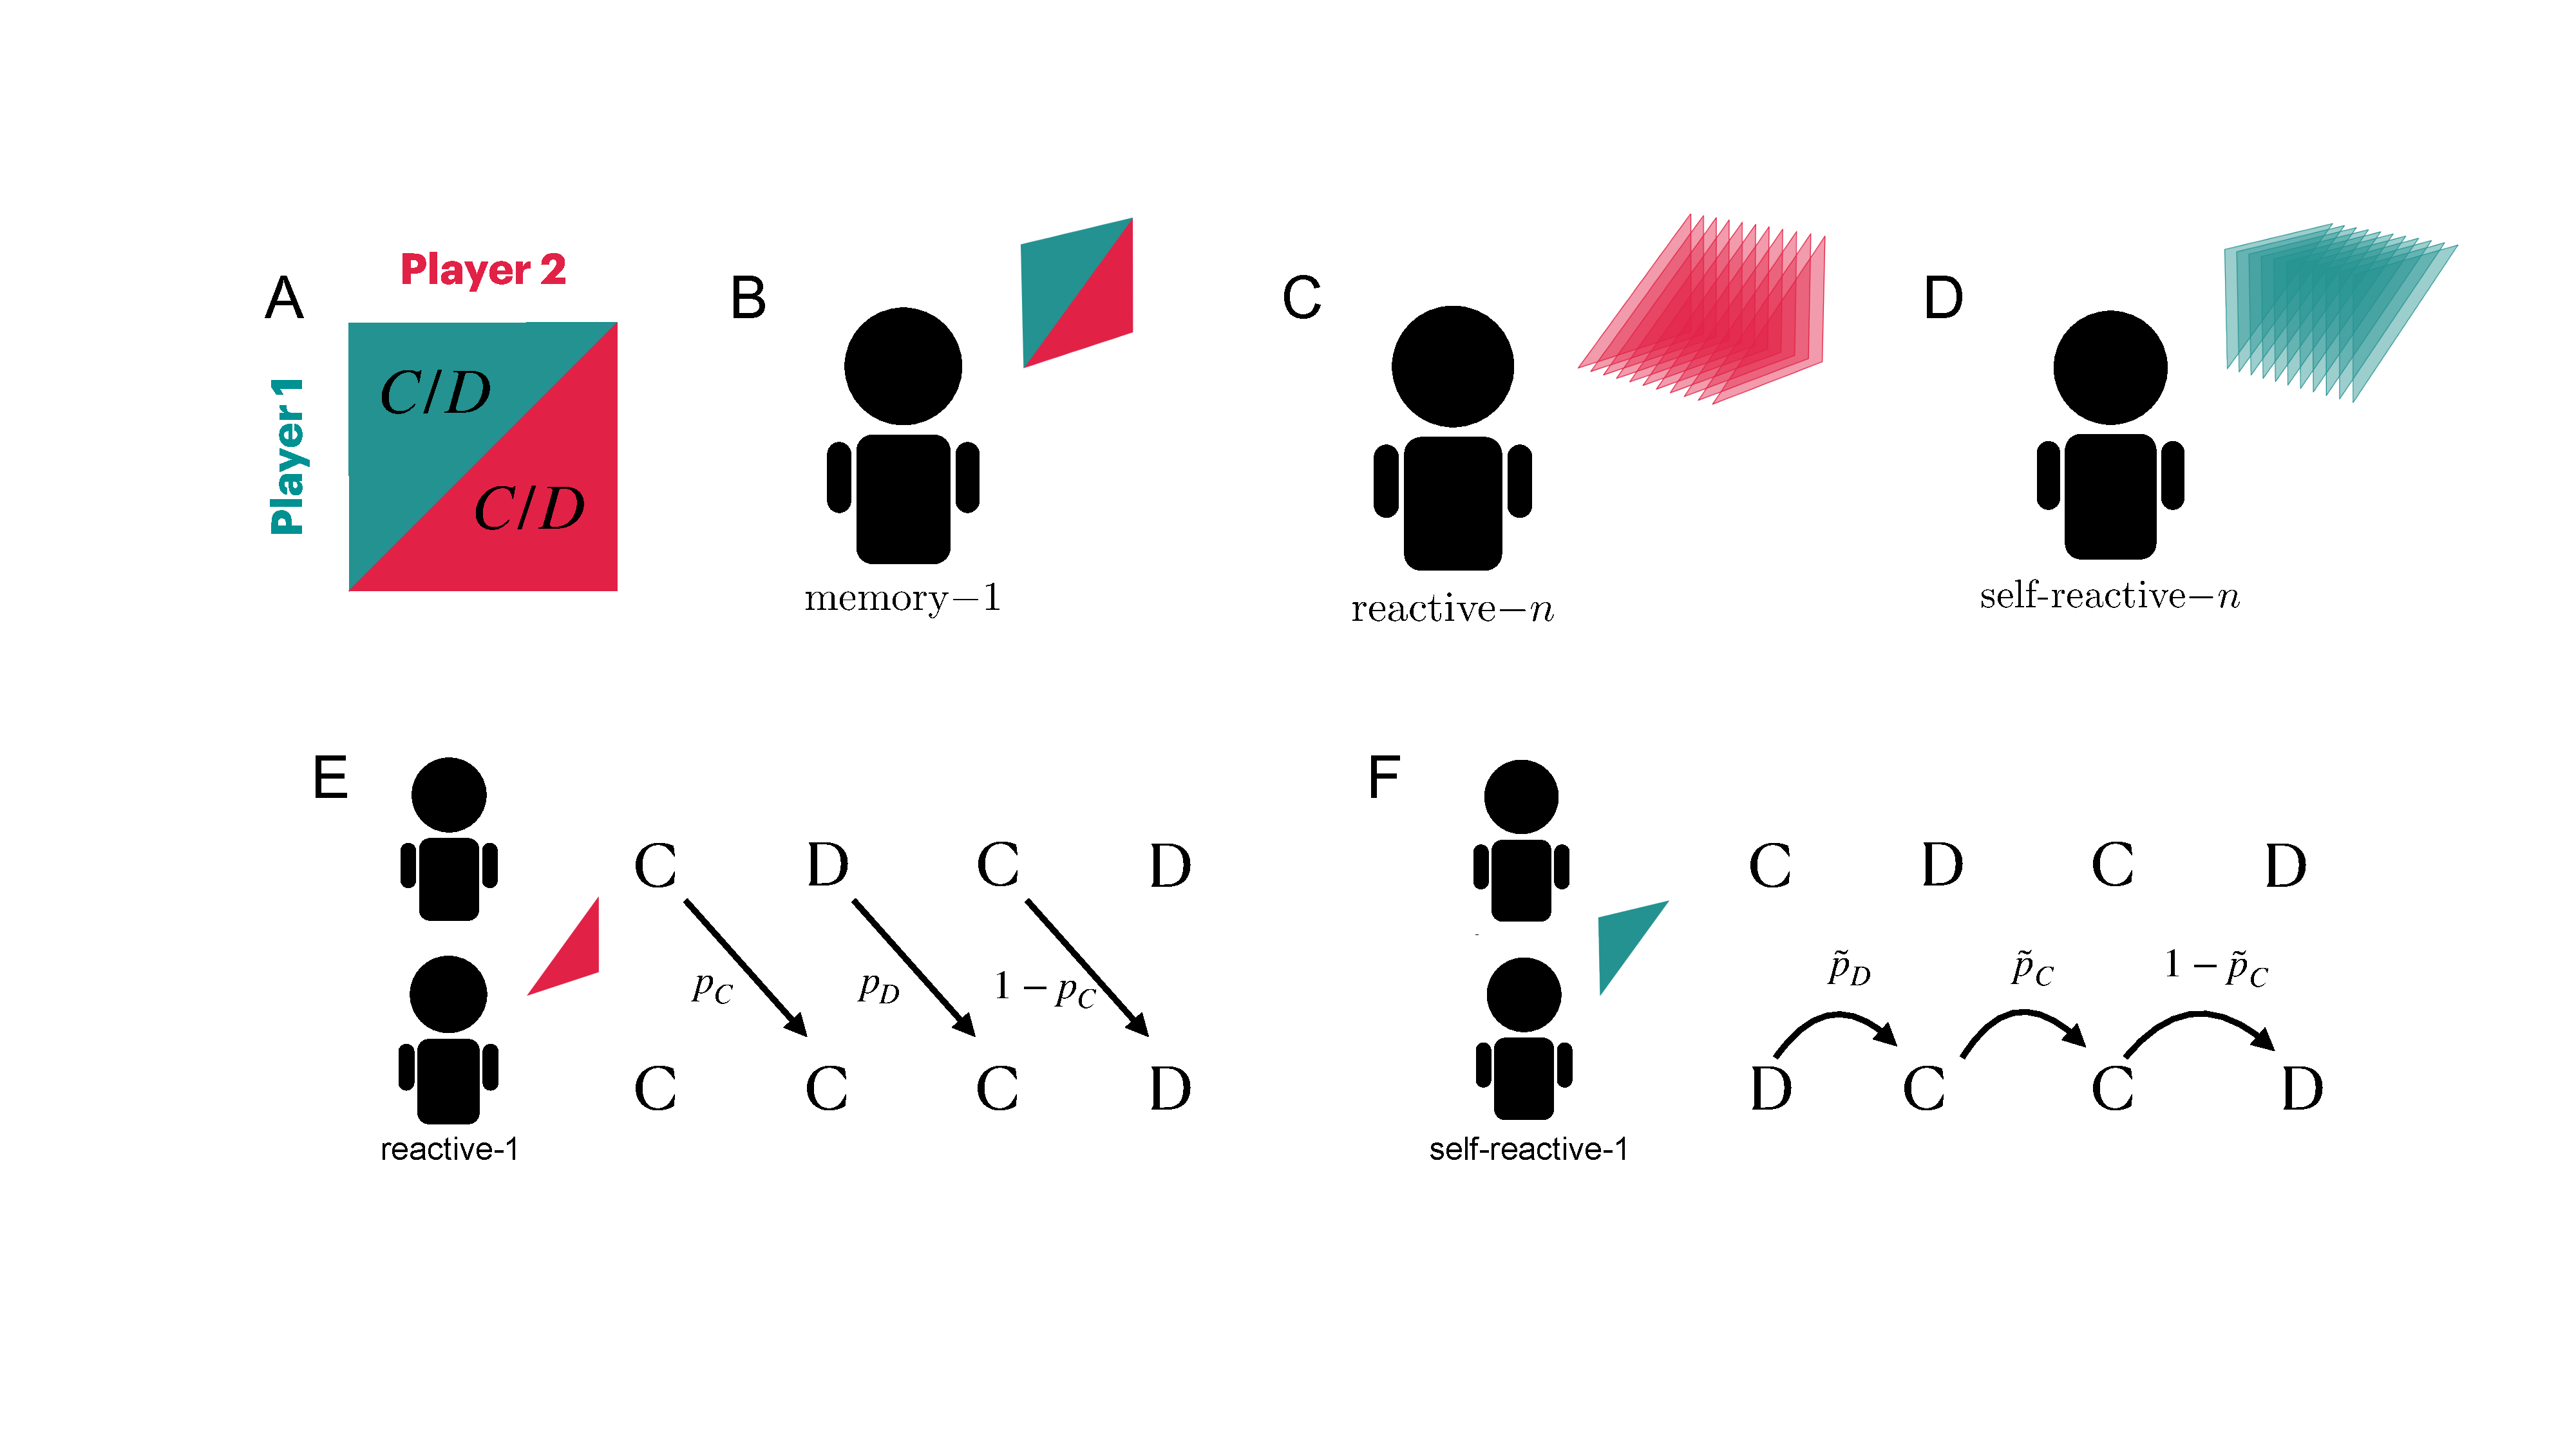
\includegraphics[width=\textwidth]{figures/conceptual_figure_model.pdf}
    \caption{Conceptual figure model.}
\end{figure}

\section{Results}

\end{document}